\normaltrue
\correctiontrue

%\UPSTIidClasse{11} % 11 sup, 12 spé
%\newcommand{\UPSTIidClasse}{12}

%\section{Rotation simple} %\label{B2:12:01}
\exer{Mouvement R  $\star$ \label{B2:13:02}}
\setcounter{numques}{0}

\UPSTIcompetence[2]{B2-13}

\index{Compétence B2-13}
\index{Mécanisme à 1 rotation}
\ifcorrection
\else
\textbf{Pas de corrigé pour cet exercice.}
\fi

\ifprof
\else
Soit le mécanisme suivant. On a $\vect{AB}=R\vect{i_1}$ avec $R=\SI{20}{mm}$. 
\begin{center}
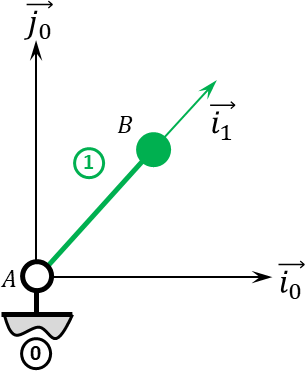
\includegraphics[width=.8\linewidth]{02_R_01}
\end{center}
\fi

\question{Déterminer $\vectv{B}{1}{0}$ par dérivation vectorielle.}
\ifprof ~\\
$\vectv{B}{1}{0}$ $ = \deriv{\vect{AB}}{\rep{0}}$ $=\deriv{R\vect{i_1}}{\rep{0}}$.
Or $\deriv{\vi{1}}{\rep{0}} = \deriv{\vi{1}}{\rep{1}} + \vecto{1}{0}\wedge \vi{1} $ $=\vect{0}+\dot{\theta}\vk{0}\wedge \vi{1}$ $=\dot{\theta}\vj{1}$.

D'où $\vectv{B}{1}{0}=R\dot{\theta}\vj{1}$.
\else
\fi

\question{Déterminer $\vectv{B}{1}{0}$ par une autre méthode.}
\ifprof ~\\
$\babarv{B}{A}{1}{0}$ $=\vect{0}-R\vi{1}\wedge \dot{\theta}\vk{0} =R\dot{\theta}\vj{1} $.

\else
\fi

\question{Donner le torseur cinématique $\torseurcin{V}{1}{0}$ au point $B$.}
\ifprof ~\\
On a directement $\torseurcin{V}{1}{0} = \torseurl{\dot{\theta}\vk{0}}{R\dot{\theta}\vj{1}}{B}$.
\else
\fi

\question{Déterminer $\vectg{B}{1}{0}$.}
\ifprof ~\\
 $\vectg{B}{1}{0} = \deriv{\vectv{B}{1}{0}}{\rep{0}}=R\ddot{\theta}\vj{1}-R\dot{\theta}^2\vi{1}$.
(En effet,  $\deriv{\vj{1}}{\rep{0}} = \deriv{\vj{1}}{\rep{1}} + \vecto{1}{0}\wedge \vj{1} $ $=\vect{0}+\dot{\theta}\vk{0}\wedge \vj{1}$ $=-\dot{\theta}\vi{1}$.)
 
\else
\fi


\ifprof
\else
\footnotesize
\begin{center}
\begin{tabular}{|p{.9\linewidth}|}
\hline
Indications :
\begin{enumerate}
\item $\vectv{B}{1}{0}=R\dot{\theta}\vj{1}$.
\item $\vectv{B}{1}{0}=R\dot{\theta}\vj{1}$.
\item $\torseurcin{V}{1}{0} = \torseurl{\dot{\theta}\vk{0}}{R\dot{\theta}\vj{1}}{B}$.
\item  $\vectg{B}{1}{0} = R\ddot{\theta}\vj{1}-R\dot{\theta}^2\vi{1}$.
\end{enumerate} \\ \hline
\end{tabular}
\end{center}
\normalsize

\begin{flushright}
\footnotesize{Corrigé  voir \ref{B2:13:02}.}
\end{flushright}%
\fi